\chapter{Correctness}
\label{chap:correctness}

One of the two fundamental issues in designing algorithms is \textit{correctness}. In this chapter, we will explore techniques to show and prove the correctness of algorithms.

\section{Defining correctness}
Your notion of correctness might be based on your experience writing code in your introductory CS classes, where you think that your code is correct as long as it matches with the sample output given, or as long as your program does not crash or go to an infinite loop.

However for this course, we would like to make a distinction between empirical correctness and provable correctness.

Simply put, we say that an algorithm is \textit{empirically correct} if it produces the correct output for every input that you only tested or practically use. More often than not, your set of inputs is just a proper subset of all the possible inputs, which is not exhaustive enough if you want to assert the correctness of the algorithm. Since you do not tend to use inputs involving edge cases, you will never know how the algorithm behaves when given unexpected inputs.

On the other hand, we say that an algorithm is \textit{provably correct} if it produces the correct output for every possible input. This does not mean you have exhaustively tested the algorithm for each and every possible input, because that is simply impractical to do. Instead, it means that you have a proof that the algorithm returns the correct output for every input.

We can have the following definition of algorithmic correctness:
\begin{definition}{(\cite{cormen_introduction_2009})}
An algorithm is said to be correct if, for every input instance, it halts with the correct output.
\end{definition}

Why should we care whether or not an algorithm is provably correct? From our experience, we design algorithms such that we know they work given reasonable inputs. But the end-users of these algorithms may not give reasonable inputs all the time.

\begin{example}[A crappy analogy, literally, sort of...]
Consider a chocolate fountain. It takes in melted chocolate as input. The manufacturer guarantees that the chocolate fountain will operate and work properly as intended, provided that it only uses melted chocolate.

\begin{figure}[H]
    \centering
    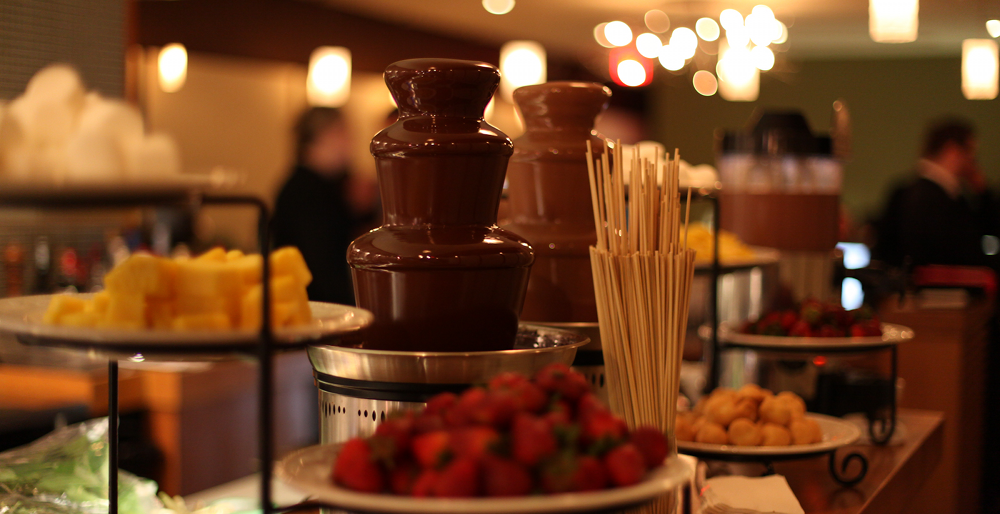
\includegraphics[width=12cm]{figures/Chocolate-Fountains.png}
    \caption{When set up properly, a chocolate fountain can be a perfect party piece}
    % \label{fig:my_label}
\end{figure}

What if the end-user somehow screwed up while operating the chocolate fountain, and a small amount of water made its way through the melted chocolate? Well, it suddenly looks unappetizing... Ew.

\begin{figure}[H]
    \centering
    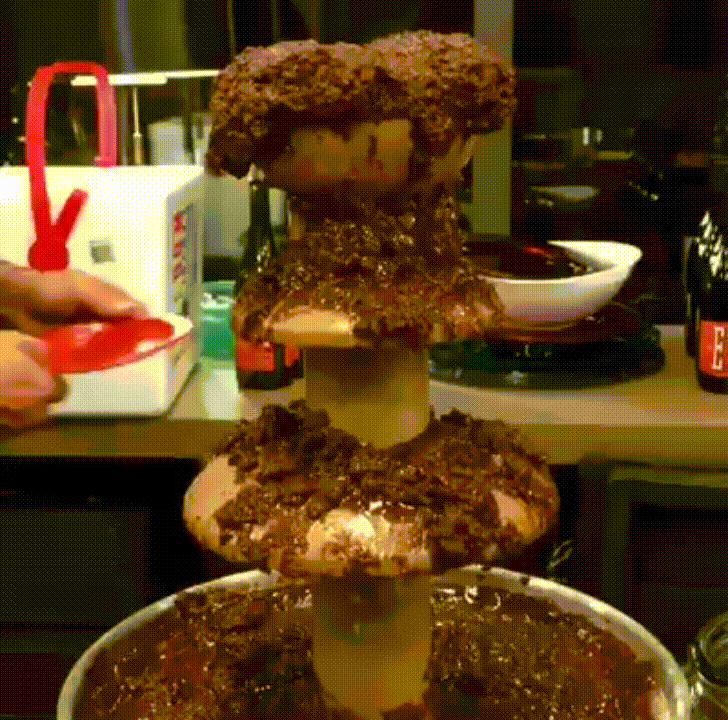
\includegraphics[width=8cm]{figures/fountain_fail.png}
    \caption{Instant disaster, just add water! (View the GIF here: \url{https://i.imgur.com/OX7Gg3R.gifv})}
    % \label{fig:my_label}
\end{figure}

It turns out water and melted chocolate don't mix. What basically happened is that the melted chocolate has seized, meaning the chocolate has clumped together to form chunks. As a result, the chocolate fountain cannot efficiently pump out the chocolate as smoothly like it did previously.

In this case, the end-user cannot complain to the manufacturer that the chocolate fountain is defective, just because it cannot pump the seized chocolate. 
\end{example}

When designing algorithms, we want to ensure that every possible inputs are all accounted for, even edge cases, and in the event that the algorithm gets an unexpected input, it should have been dealt with accordingly. We do not want an algorithm to behave unexpectedly or inconsistently when given unexpected input.

By ensuring that an algorithm is provably correct, we avoid unexpected or undefined behavior. Thus, we ensure that an algorithm \textit{expectedly} returns the correct output.

\section{Mathematical induction}
One technique to prove the correctness of an algorithm is through a proof by induction. This is commonly used when an algorithm only involves a closed-form expression.

Recall that there is a neat formula to get the sum of integers from $1$ to $n$, which is as follows:
\[
\sum_{i=1}^{n} i = \frac{n\left(n+1\right)}{2}
\]

How are we sure that this formula gives the correct answer for all positive integers $n$?

\begin{claim}
The above formula gives the correct answer for integers $n>0$.
\end{claim}

\section{Loop invariants}
How do loops work anyway? Recall that a loop consists of a condition, and a series of statements. These statements are always executed, so long as the loop condition holds true. Once the loop condition does not hold anymore, the loop terminates without executing the statements.

If for each iteration, everything inside the loop gets executed, then there must be some condition that holds true at the start of every iteration. Furthermore, the statements inside the loop must make sure that this condition will still hold at the start of the next iteration. This condition is what we call a \textit{loop invariant}. We use loop invariants to prove the correctness of iterative algorithms.

\begin{definition}
A loop invariant is a statement that remains true before, during, and after every iteration of the loop. It satisfies these properties:
\begin{enumerate}
    \item Initialization: A loop invariant is true at the start of the loop.
    \item Maintenance: If a loop invariant is true before the $i$th iteration, it should also remain true before the $\left(i+1\right)$th iteration.
    \item Termination: A loop invariant is true after the loop ends, which helps us show that the algorithm is correct.
\end{enumerate}
\end{definition}

How do we find a loop invariant? One way is to consider what happens in each iteration of the loop. Try looking at how the value of the variables change throughout an iteration.
\begin{exercises}

[to-do]
\end{exercises}